\documentclass[8pt]{beamer}
\usepackage{lmodern}  % Optional: Improves font quality
%\renewcommand{\familydefault}{\rmdefault}  % Set default font to serif
\usetheme{default} % Very simple theme
\usecolortheme{dove} % Minimalist grayscale colors
\setbeamertemplate{navigation symbols}{} % Remove navigation bar

\usepackage{graphicx} % Package for images
\graphicspath{{figs/}} % Path to your figures directory
\usepackage{array}  % For better column spacing
\usepackage{caption} % Required for \captionof
\usepackage{natbib}
%\addbibresource{references.bib}  % Load your bibliography file
% Title Information
\title{Stochastic methods in water resources}
\subtitle{Lecture 2: Descriptive statistics, univariate and bivariate statistics}
\author{Luis Alejandro Morales, Ph.D.}
\institute{Universidad Nacional de Colombia} %// Department of Civil and Agriculture Engineering}
\date{\today}

\begin{document}

% Title Slide
\begin{frame}
    \titlepage
\end{frame}

%-------- from Kotte and Vujica
\section{Hydrologic data}

\begin{frame}{Definitions}
    \begin{itemize}
        \item \alert{Random variable}: A measured quantity with inherent randomness and uncertainty.
        \item \alert{Data population}:  Constitute the universe of possible values that a variable can take.
        \item \alert{Data sample}: A representative data set of population. E.g. observed streamflow at Calamar's IDEAM station at the Magdalena River.
        \item \alert{Distribution}: Pattern of variability of a random variable in the frequency space. 
        \item \alert{Continuous variable}: A variable that can take any values on a continuous scale. E.g. streamflow in m$^3$ s$^{-1}$.
        \item \alert{Discrete variable}: A variable that can take certain values (e.g. integers). E.g. number of days per month with no rain at the Dorado's airport station.
       
    \end{itemize}

Data is analysed on \alert{data sample} which is . Statistical and probabilistic analysis of samples serve to make \alert{inferences} on the data population.
\end{frame}
\begin{frame}{Hydrologic data}
    \begin{block}{Data types}
        Hydrologic data relate to water quantity and quality acquired in time and space; these data is also called \alert{variable}. Four types are identified:
        \begin{enumerate}
            \item \alert{Historic or chronology data}: Data observed continuously or discretely in time from any process that result in a time series. Most of the hydrologic data is of this type. E.g. gauge rainfall station. 
            \item \alert{Observations in space}: Data observed across an line, area or specific space. E.g. sediment characteristics across a river bed.
            \item \alert{Laboratory or field experiment data}: Data acquired controlling esternal factors. Used in basic and applied research. 
            \item \alert{Simultaneous measurements}: Simultaneous measurements of two or more variables in order to stablish relationships among them.
        \end{enumerate}
    \end{block}    
\end{frame}
\begin{frame}{Hydrologic data}
    \begin{block}{Quality of data}
        Some generalities about quality of data:
        \begin{itemize}
            \item The \alert{true value} of any observation is never known because there are unavoidable errors in the process of data acquisition.
            \item \alert{Observed values} are acquired through multiple surveys, recordings or experiments.
            \item Errors in observed data occur during: \alert{sensing/measuring}, \alert{transmitting}, \alert{recording/saving} and \alert{processing}. 
            \item Data errors can be \alert{random} or \alert{systematic}. Random errors are always present while systematic errors means \alert{inconsistent data} (e.g. no calibrated manometer cause a consistent positive bias). \alert{Non-homogeneous data} are due to errors induced by accidents, nature changes, human activities; also known as non-stationary data (e.g. forest fire changes basin functioning). 
            \item Random errors has approximately a \alert{Gaussian distribution} and the \alert{standard deviation} indicate the magnitude of the errors.
            \item Any rigorous analysis and future projection of a hydrological variables must be based on data free of significant inconsistency and non-homogeneity, with acceptable random errors. 
        \end{itemize}
    \end{block}
\end{frame}

%--------
\section{Univariate statistics}
\subsection{Graphical representation}
\begin{frame}{Graphical representation}
    The first step in the analysis of data is its representation. One kind of representation is \emph{graphical} representation. This provides insights into the form and shape of data leading to preliminary understanding of the generating process. Graphical representation types are:

    \begin{minipage}{0.49\textwidth}{\alert{Bar chart}}
        Representation of the data where in the $x$ axis we have the values of the discrete variable and the occurrence are represented by the heights ($y$) of the bars. 
    % Ex 1.1. Kotte
    \begin{exampleblock}{Flood ocurrence}
        Consider the number of floods per year for a period of 34 years in the Magra River at Calamazza, located between Pisa and Genoa. A flood occurs when mean daily streamflows overcome a threshold.  
    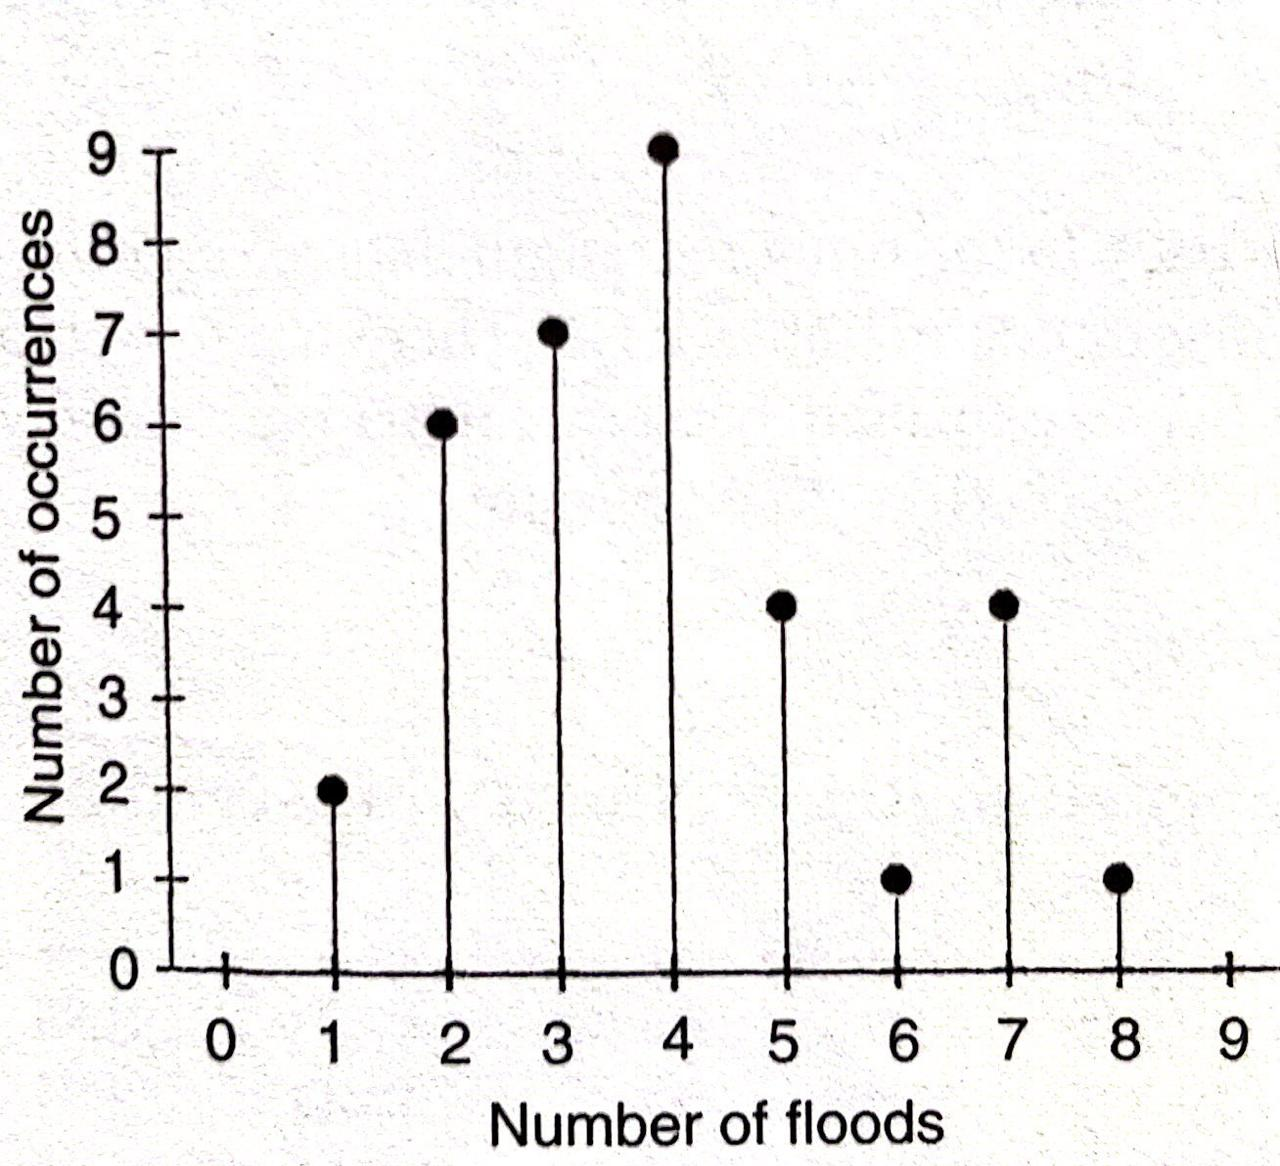
\includegraphics[width=0.9\textwidth]{fi111.jpeg}
    The figure shows a symmetrical behaviour of floods with a mid-location close to 4 floods per year.
    \end{exampleblock}
\end{minipage}
\hfill
\begin{minipage}{0.495\textwidth}{\alert{Dot diagram}}
Continuous data can be represented on a single axis when the data set is small. 
    \begin{exampleblock}{Drought index}
       The meteorological drought index estimated based on monthly precipitation time series in the last 25 years is show in the figure. Note that the data is sorted in ascending order. 
    %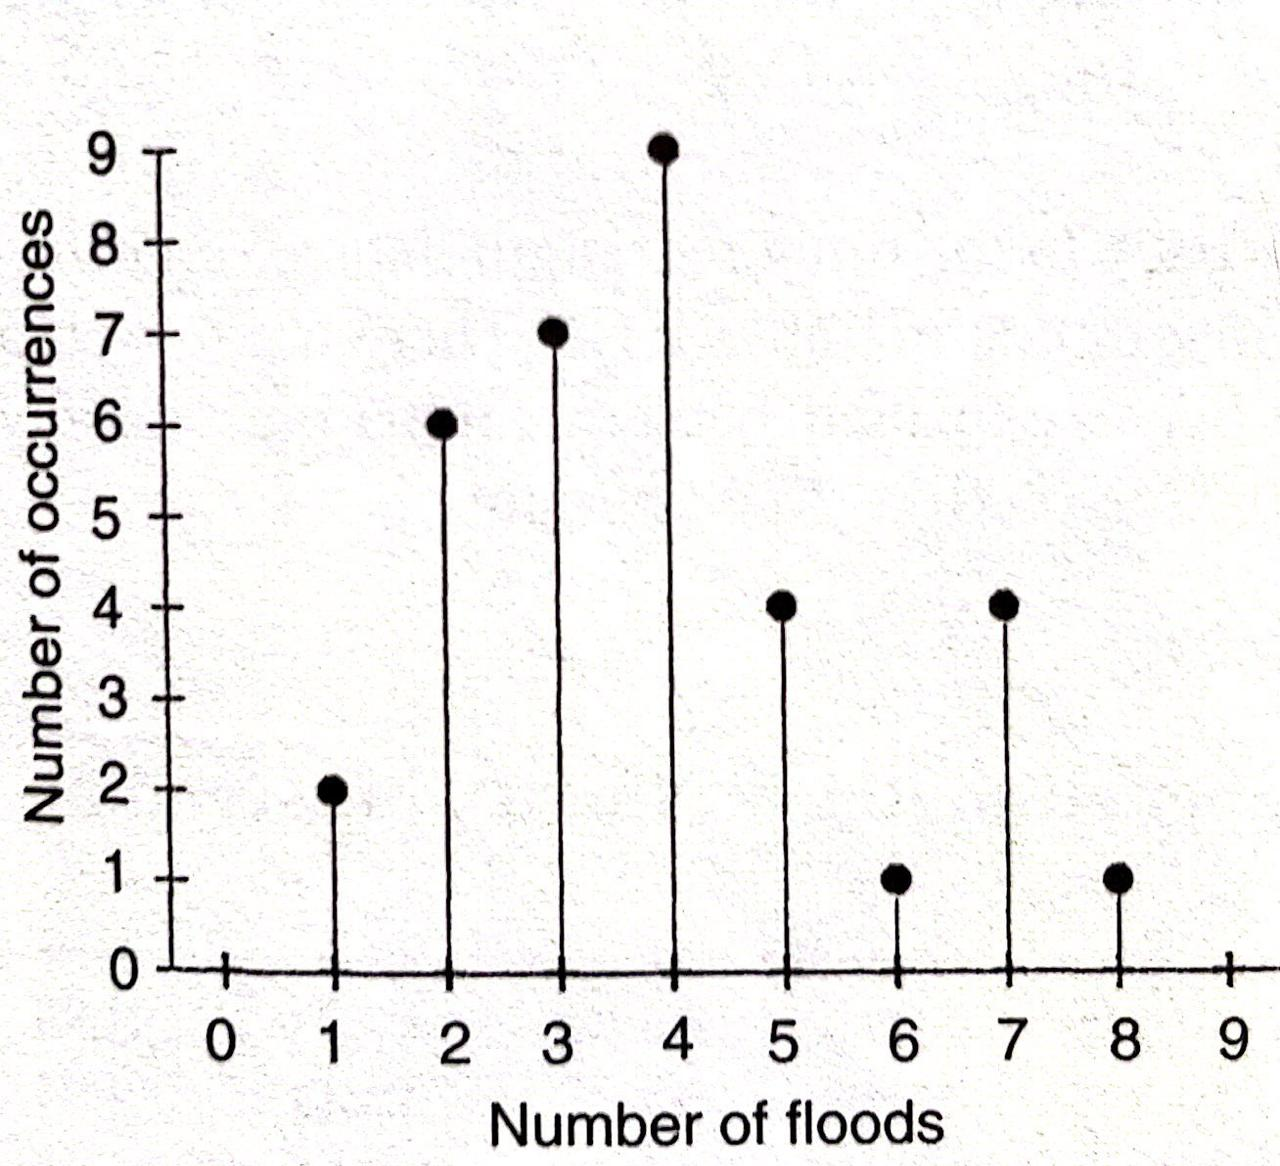
\includegraphics[width=0.9\textwidth]{fi111.png}
    The plot shows the spread of the drought index and approximately the mean value.
    \end{exampleblock}
\end{minipage}
\end{frame}

\begin{frame}{Graphical representation: Histogram}
        When data set is greater than 25 observations, data can be represented based on their frequency of occurrence. The data set can be discrete or continuous. This graphical representation of data in the frequency domain is known as \emph{histogram}. To plot a histogram:
        \begin{enumerate}
            \item Sort the data in ascending order $x{min}\cdots x_{max}$.
            \item Estimate the data range ($r$) as $r = x_{max} - x_{min} $.
            \item The data is initially divided  into groups or classes ($n_c$) according to the data magnitude where each group has a lower and upper limit.  According to Sturges (1926), $n_c = 1 + 3.3 \log_10 n $, donde $n$ is the number of data. Note that $n_c$ must be an positive integer and is recommended that $5 \le n_c \le 25$. $n_c$ can be estimated using Freedman and Diaconis (1981) formula  $n_c = \frac{r n^{1/3}}{2\left(Q_3 - Q_1\right)}$, where $Q_3$ is the median of the upper half of the data and $Q_1$ is the median of the lower half of the data. The difference $Q_3 - Q_1$ is known as the \emph{interquartile range}.
            \item Establish the lower and the upper limits of each class.
            \item Count the number of data occurrence within each class (frequency).
            \item Plot the histogram where in the x-axis there is the limits of the $n_c$ classes and the y-axis the frequency. Frequency can be expressed as a \emph{relative frequency} which is, for each class, the frequency divided by $n$. Note that the sum of all relative frequencies is equal to 1, so the relative frequency indicate the chances of occurrence of certain values of $x$.
\end{enumerate}
\end{frame}

\begin{frame}{Graphical representation: Histogram}
    Instead of bars of fixed width to plot the histogram, the data can be represented as a \emph{polygon line}. This polygon line joins the middle point of each bar and indicate approximately the distribuition of $x$. \\
    \begin{minipage}{0.495\textwidth}
    \begin{exampleblock}{Annual precipitation}
        Consider the annual precipitation in Seattle, Washington, US between 1948 and 2015. The following figure show the histogram for the data. Note that the most frequent precipitation is between 35 and 40 inches and that the bell shape of the histogram. 
    \end{exampleblock}
\end{minipage}
\hfill
\begin{minipage}{0.495\textwidth}
    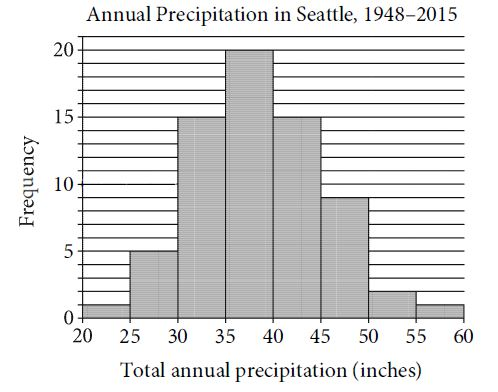
\includegraphics[width=0.95\textwidth]{fie1.JPG}
\end{minipage}\\
As $n \to \infty$, the class width tend to decrease and polygon line becomes a curve that represent the \emph{probability density function (pdf)} of the population of $x$. 
\end{frame}

\begin{frame}{Graphical representation: Cumulative frequency curve}
    \begin{itemize}
        \item If the frequency or the relative frequency is accumulated from the smallest class to the largest classes, it is possible to plot the cumulative frequency against the middle point of the classes to form \emph{cummulative frequency curve} or the \emph{cumulative relative frequency curve}. 
        \item Note that the classes middle point in acceding order is represented in the x-axis while the cumulative frequency is in the y-axis. 
        \item The  y-axis represent the probability of nonexceedance of a value of $x$ showed in the x-axis. 
        \item The cumulative relative frequency are between 0 and 1. 
        \item This curve yields important information such as the \emph{quartiles}, which is the division of the total frequency domain in 4, including the \emph{median} ($Q_{50}$). 
        \item In general the frequency domain can be divided into $n-1$ to get the \emph{quantiles}. A cumulative frequency polygon is known as the \emph{Q-plot}. 
        \item As $n \to \infty$, the class width tend to decrease and the cumulative frequency curve becomes the \emph{cumulative distribution function (cdf)} of the population of $x$. 
    \end{itemize}
    \begin{minipage}{0.495\textwidth}
    \begin{exampleblock}{Air temperature}
        Consider mean hourly air temperature during the day and during the night at the Timau National Observatory, Indonesia \citep{priyatikanto2024weather}. The plot shows the histograms and the cummulative relative frequency curves for air temperature data at night and during the day. Note that the histogram are centered around a mid value and bid skewed toward the right. 
    \end{exampleblock}
\end{minipage}
\hfill
\begin{minipage}{0.495\textwidth}
    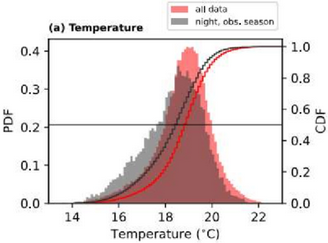
\includegraphics[width=0.95\textwidth]{fie2.png}
\end{minipage}
\end{frame}

\begin{frame}{Graphical representation: Duration curve}
    \begin{itemize}
        \item \emph{Duration curves} are useful tools for the design and planning in water resources engineering. 
        \item In River Engineering is common to obtain the \emph{flow duration curve} based on streamflow records. 
        \item The flow duration curve is a cumulative frequency curve where the y-axis represent the time (e.g. days) during which the flow is exceeded or the percentage of time the flow is exceeded. 
    \end{itemize}
    \begin{minipage}{0.495\textwidth}
    % Ex 1.6. Kotte
    \begin{exampleblock}{Streamflow duration}
        The figure shows the flow duration curve of the Dora Riparia River in the Italian Alps estimated for a period of 47 years. If for example, it is needed to divert flow when $10 < Q < 20$, the durantion curve can be analysed to extract the number of days when $Q$ exceed the streamflow limits and estimate the numerical integral to compute the area under the duration curve \citep{kottegoda2008applied}.
    \end{exampleblock}
\end{minipage}
\hfill
\begin{minipage}{0.495\textwidth}
    %\includegraphics[width=0.95\textwidth]{fi117.png}
\end{minipage}
\end{frame}

\subsection{Numerical summaries of data}
\begin{frame}{Numerical summaries of data}
    A part from graphical representation of data sets, data information can be conveyed in a efficient and precise manner. This includes numerical values that caracterized the data and highlight their main features that can be visualized in the histogram and in the cumulative frequency curve. This numerical summaries are useful for \emph{statistical inferences}. There are three types of numerical values:
    \begin{itemize}
       \item \emph{Measures of central tendency}
       \item \emph{Measures of dispersion} 
       \item \emph{Measures of asymmetry} 
    \end{itemize}
\end{frame}

\begin{frame}{Measures of central tendency}
    Data sets from diverse sources tend to cluster around a \emph{central value} of $x$, which is representative of the sample; this is known as \emph{central tendency}. There are three types of measures to estimate a central value: \emph{the mean}, \emph{the mode} and \emph{the median}. The chosen of them depends on the use of the central value.
    \begin{block}{Sample arithmetic mean}
    For a dada sample $x_1, x_2, \cdots, x_n$ of size $n$ de una variable $x$, the sample arithmetic mean ($\bar{x}$):
      $$
      \bar{x} = \frac{1}{n} \sum_{i=1}^n x_i
      $$
      The mean is perhaps the most basic measures to represent the data and to represent the central tendency location. As a matter of convention, $\mu$ represent the \emph{population mean}. $\bar{x}$ can be affected by low and/or high values of $x$ which are know as \emph{outliers}. This unexpected values can results from faulty instruments or errors induced by the environment or by human beings and must be revised carefully in order to eliminate them to avoid a misleading computation of $\bar{x}$. In some cases, there are values that have a higher weight than others within the sample of $x$, so the \emph{weighted mean} can be calculated as $ \bar{x}_w = \frac{\sum_{i=1}^n w_i x_i}{ \sum_{i=1}^n w_i}$ where $w_i$ is the weight of the value $x_i$. The estimation of $w_i$ is quite difficult and subjective.  
    \end{block}
\end{frame}

\begin{frame}{Measures of central tendency}
    \begin{block}{Sample median}
        The \emph{median} ($x_m$) is the value in the middle of a ordered sample of $x$ when $n$ is odd. When $n$ is even, it is the average of the two central values in the ordered sample. In comparison with the mean, the median is slightly affected by outliers so it is known as the \emph{resistant measure}. From the cumulative relative frequency curve ($F_X$), the median corresponds to the $x$ values for which the cumulative relative frequency is equal to 0.5.  
    \end{block}

    \begin{block}{Sample mode}
        The \emph{mode} is the most frequent value within the sample of $x$. However in some cases, there is not a unique most frequent value, so it must be obtained by analysing the histogram or the cumulative frequency curve. In cases where asymmetry of data increase, the mode becomes more useful than the mean and the median. Also, as the data sample increases, the mode tends to be the peak of the histogram.  
    \end{block}
    Other central tendency measure is the \emph{geometric mean} that is estimated as $\bar{x}_g = e^{\frac{1}{n} \sum_{i=1}^n \log x_i}$ and it can be useful when the data sample has a positive asymmetry. 

    \centering
    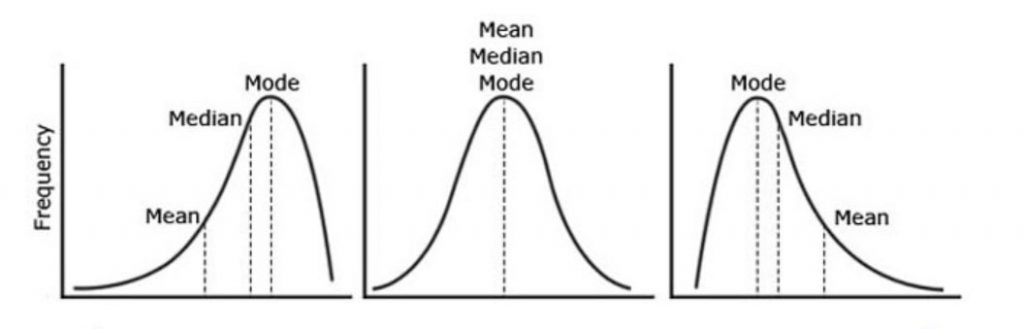
\includegraphics[width=0.98\textwidth]{fie3.JPG}
\end{frame}

\begin{frame}{Measures of dispersion}
    The \emph{measure of dispersion} represents the degree of scatter of the observations. This shows the variability of the observed phenomena and thus the precision of the data. There area methods to quantify the dispersion in a data sample.

    \begin{block}{Sample range}
        After sorting the sample data, the \emph{range} ($r$) can be computed as $r = x_{max} - x_{min}$. Since dispersion reduce after sample size increases, the range is unaffected by that, so that this is considered  a poorly measure of the dispersion. Also, as it is computed based on the extreme values, other values does not play a role in this estimation. The  \emph{interquartile range} defined as $Q_3 - Q_1$,  where $Q_3$ is the median of the upper half of the data and $Q_1$ is the median of the lower half of the data, is thus more appropriate because this is a relatively resistant measure.
    \end{block}

    \begin{block}{Sample mean absolute deviation}
        Range as well as interquartile range ignore certain amount of data. This can be corrected if the deviation of each observation with respect to a central measure (e.g. $\bar{x}$) is computed. The \emph{mean absolute deviation} is thus estimated as:
        $$
        d = \frac{1}{n}\sum_{i=1}^n | x_i - \bar{x} |
        $$
    \end{block}
\end{frame}

\begin{frame}{Measures of dispersion}

    \begin{block}{Sample variance and standard deviation}
        The \emph{variance} of the sample is the most representative estimate of the population dispersion and is calculated as:
        $$
        s^2 = \frac{1}{n} \sum_{i=1}^n \left( x_i - \bar{x} \right)^2
        $$
        and the square rood of the variance is known as the \emph{standard deviation} ($s$):
        $$
        s = \sqrt{\frac{1}{n} \sum_{i=1}^n \left( x_i - \bar{x} \right)^2}
        $$
        where $s$ has the same units of $x$. In contrast to \emph{mean absolute deviation}, the standard deviation is very influenced by small and large values; note that standard deviation of the population is known as $\sigma_X$. To get a non bias estimator of $\sigma_X$, $\hat{s}$ is estimated as:
        $$
        \hat{s} = \sqrt{\frac{1}{n-1} \sum_{i=1}^n \left( x_i - \bar{x} \right)^2}
        $$
        
    \end{block}
\end{frame}

\begin{frame}{Measures of dispersion}

    \begin{block}{Sample variance and standard deviation}
        A dimensionless measure of the dispersion can be estimated using the concept of \emph{sample coefficient of variation} computed as $v = \frac{s}{\bar{x}}$ and can be expressed as a percentage. Note that an \emph{estimator} refers to a method to estimated a constant of a parent population, so for instance $\bar{x}$ and $s$ are estimators of $\mu$ and $\sigma$, respectively. This means that $\bar{x}$ and $s$ are estimates of the true values and the average of these estimators tend to the population values. 

        \centering
        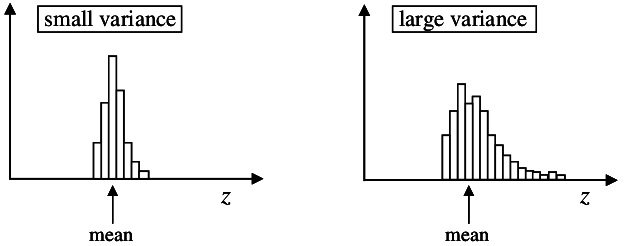
\includegraphics[width=0.98\textwidth]{fiBi25.png}
        \captionof{figure}{Histogram of a data sample with the same $\bar{x}$ and different variance (taken from \cite{bierkens2007})}
    \end{block}
\end{frame}

\begin{frame}{Measure of asymmetry}
    An important property of the histogram or the frequency curve  is its shape with respect to a symmetry axis (e.g. the mode).

    \begin{block}{sample coefficient of skewness}
        The \emph{coefficient of skewness} ($g_1$) measure the asymmetry of the data set with respect to its mean. For a data sample $x_1, x_2, \cdots, x_n$ of size $n$ of a variable $x$, the coefficient is computed as:
        $$
        g_1 = \frac{\sum_{i=1}^n \left(x_i - \bar{x} \right)^3}{n s^3}
        $$
        Note that $s$ is the standard deviation and $g_1$ is dimensionless. $g_1$ can be affected by outliers. Observing a histogram, the data set is positively skewed ($g_1 > 0$)  is the longest tail is on the right and negatively skewed ($g_1 < 0$) if the longest tail is on the left. 

        \vspace{-0.1cm}
        \begin{center}
        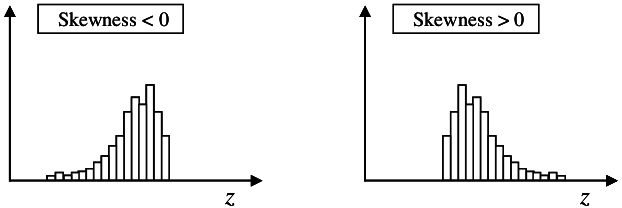
\includegraphics[width=0.98\textwidth]{fiBi26.png}
        \vspace{-0.3cm}
        \captionof{figure}{Histogram of a data sample with the same $s^2$ and different skewness (taken from \cite{bierkens2007})}
        \end{center}
        \vspace{-0.3cm}
        A positively skewed histogram implies: mode $<$ median $<$ mean,  while a negatively skewed histogram implies: mean $<$ median $<$ mode.
    \end{block}
\end{frame}

\begin{frame}{Measure of asymmetry}
    A resistant measure of the asymmetry can be estimated based on the quantiles ($Q_q$) or percentiles ($Q_q/100$). A quantile ($Q_q$) is obtained from the cumulative relative frequency curve which is the value of $x$ for which the cumulative relative frequency  is equal to $q$. So for instance $Q_{0.25}$ is the value of $x$ whose cumulative relative frequency is 0.25. 
        \vspace{-0.1cm}
    \begin{center}
        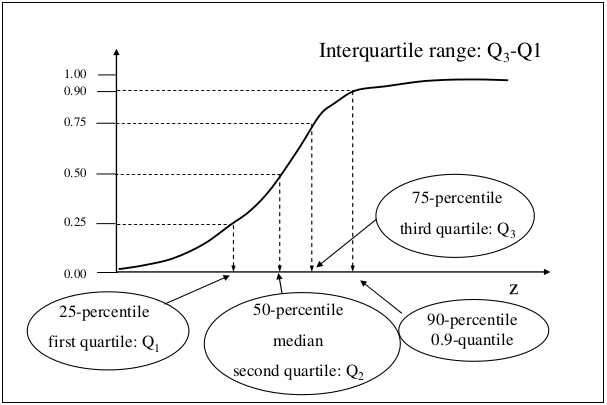
\includegraphics[width=0.7\textwidth]{fiBi29.png}
        \vspace{-0.3cm}
        \captionof{figure}{Percentiles in the cumulative frequency curve (taken from \cite{bierkens2007})}
        \end{center}
According to this, the quartile coefficient of asymmetry is:
    $$
    g_s = \frac{\left(Q_{0.75} - Q_{0.5}\right) - \left( Q_{0.5} - Q_{0.25}\right)}{Q_{0.75}-Q_{0.25}}
    $$

\end{frame}


\begin{frame}{Measure of peakedness}
The measure of the relative ascending steepness nearby the mode in the histogram or in the frequency curve is said to be a measure of the peakedness.
    \begin{block}{Sample coefficient of kurtosis}
        The \emph{coefficient of kurtosis} ($g_2$) measure the degree of peakedness of the data set. For a data sample $x_1, x_2, \cdots, x_n$ of size $n$ of a variable $x$, the coefficient is computed as:
        $$
        g_2 = \frac{\sum_{i=1}^n \left(x_i - \bar{x} \right)^4}{n s^4}
        $$
        Note that $s$ is the standard deviation and $g_2$ is dimensionless. For \emph{Gaussian probability distribution (pdf)}, $g_2$ is equal to 3. So it is common to estimate $g_2$ with respect to a Gaussian pdf, so that, the equation for $g_2$ becomes:
        $$
        g_2 = \frac{\sum_{i=1}^n \left(x_i - \bar{x} \right)^4}{n s^4} - 3
        $$

        \vspace{-0.3cm}
        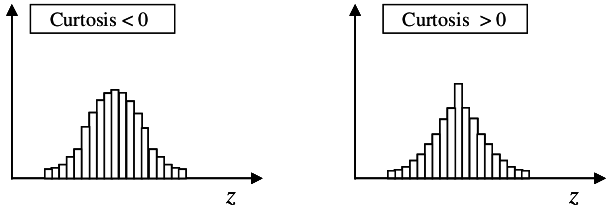
\includegraphics[width=0.95\textwidth]{fiBi27.png}
        \vspace{-0.3cm}
        \captionof{figure}{Histogram of a data sample with negative and positive kurtosis (taken from \cite{bierkens2007})}
    \end{block}
\end{frame}

\subsection{Exploratory data analysis}
\begin{frame}{Exploratory data analysis}
Exploratory data analysis is a manner to graphycally represent data  compactely. Usually, this analysis does no obey to any particular purpose or question in mind but to represent the data. Such graphic representation are made based on:
\begin{itemize}
    \item \emph{Steam-and-Leaf plot}
    \item \emph{box plot}
\end{itemize}
Because of their clarity, box plots are usually more used.
\end{frame}

\begin{frame}{Box plot}
    A box plot summarizes the main statistical features of a data set in one plot. The plot displays the percerntiles $Q_{25}$, $Q_{50}$ and $Q_{75}$ on a box aligned verticall or horizontally. Also, the minimun and the maximum values are represented by lines that extend in both directions from the box and are known as \emph{whiskers}. For a vertically aligned box plot, the main statistics from bottom to the top are: minimum, $Q_{25}$, $Q_{50}$, $Q_{75}$ and maximum. In some cases, the minimum and maximum values are replaced by percentiles $Q_{5}$ and $Q_{95}$, respectively. Box plots are useful to compare different data sample and the box width is, sometimes, proportional to the sample size.
    \vspace{-0.2cm}
        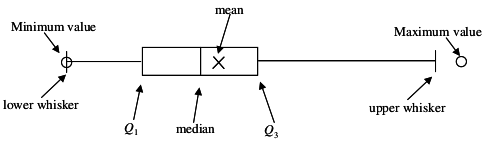
\includegraphics[width=0.95\textwidth]{fiBi210.png}
        \vspace{-0.1cm}
        \captionof{figure}{Box plot structure (taken from \cite{bierkens2007})}
        Note also that the $\bar{x}$ is somewhere between $Q_{25}$ and $Q_{75}$ and that the plot shows features of the data distribution such as the degree of data dispersion and skeweness. Box plots are useful to detect outliers, so for a vertically oriented box plot outliers are those  values above a distance $1.5Q_{75}$ and below a distance $1.5Q_{25}$. 
\end{frame}

%--------
\section{Bivariate statistics}
\begin{frame}{Sample covariance and correlation coefficients}
    When two variables are observed  is of interest to establish their relationship and association. A preliminary analysis of the relationship can be made using a \emph{scatter plot} which are pair of points $(x_i, y_i)$ of variables $x$ and $y$ represented in the cartesian plane. The behaviour of the points provide some preliminary hinds hinds about the relationship of $x$ and $y$. A better estimate of this relatioship is assesed by estimating the \emph{sample covariance coefficient} and \emph{sample correlation coefficient}.

    \begin{block}{Sample covariance coefficient}
        The sample covariance coefficient $s_{X,Y}$ shows the \emph{linear} relationship between $X$ and $Y$ and it is calculated as:
        $$
        s_{X,Y} = \frac{1}{n} \sum_{i=1}^{n} \left(x_i - \bar{x}\right)\left(y_i - \bar{y}\right)
        $$
        The greater $s_{X,Y}$, the larger the association between $X$ and $Y$ with respect to higher or lower than average values. 
   \end{block}

\end{frame}
\begin{frame}{Sample covariance and correlation coefficients}
    \begin{block}{Sample correlation coefficient}
        If the sample covariance coefficient $s_{X,Y}$ is divided by the sample standard deviation $s_X$ and $s_Y$, we have the sample correlation coefficient:
        $$
        r_{X,Y} = \frac{1}{n s_X s_Y} \sum_{i=1}^{n} \left(x_i - \bar{x}\right)\left(y_i - \bar{y}\right)
        $$
    where $-1 \le r_{X,Y} \le 1$. $r_{X,Y}$ is also known as the \emph{product-moment correlation coefficient}. In case all the points in a scatter plots are close to a straight line $y = \beta_0 + \beta_1 x$, $X$ and $Y$ are positively correlated $r_{X,Y} > 0$ (if $r_{X,Y}=\beta_1 = 1$, $X$ and $Y$ are perfectly correlated). $X$ and $Y$ are negatively correlated when $r_{X,Y} < 0$ (if $r_{X,Y}=\beta_1 =-1$, $X$ and $Y$ are perfectly correlated). It can be the case that the scatter plot does not show a linear relationship between $X$ and $Y$ but a non-linear relationship e.g. exponential or potential. In that case, a logarithm transformation of one or both variables is needed in order to determine their relationship. On the other hand, a $r_{X,Y} \approx 0$ show no relationship between $X$ and $Y$ but no independency. In general, $r_{X,Y}$ show the degree of association between $X$ and $Y$ but a cause-effect relationships necessarily. $X$ and $Y$ can have a value of $r_{X,Y}$ close to 1 or -1 because of a third variable so this does not imply a cause-effect relationship. So a relationship of the form $y = \beta_0 + \beta_1 x$ can be used to predict $Y$ (\emph{response} variables) as function of $X$ (\emph{explanatory} variable).
   \end{block}

\end{frame}

\begin{frame}{Sample covariance and correlation coefficients}
        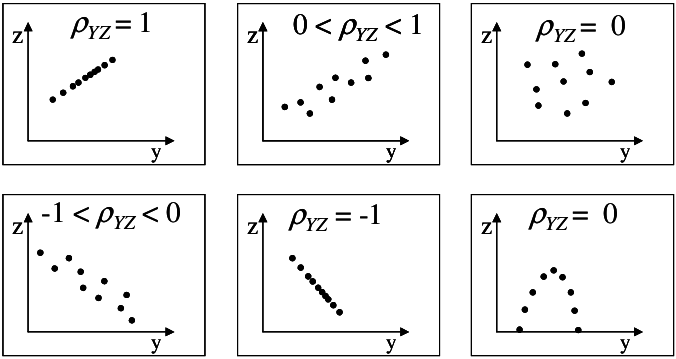
\includegraphics[width=0.95\textwidth]{fiBi213.png}
        \vspace{-0.1cm}
        \captionof{figure}{Scatter plots and $r_{X,Y}$ (taken from \cite{bierkens2007})}
\end{frame}

\begin{frame}{Q-Q plots}
    When one want to compare the probability distribution of two variables $X$ and $Y$, the quantiles of $X$ against the quantiles of $Y$ form the \emph{Q-Q plots}. Both data sets are sorted and the cummulative frecuency curve is estimated for $X$ and $Y$. The values of $X$ and $Y$ that correspond to a value of cumulative frequency are plotted to form the Q-Q plot. When the plot depart from linearity, this indicates other types of differences between the two distributions. 
    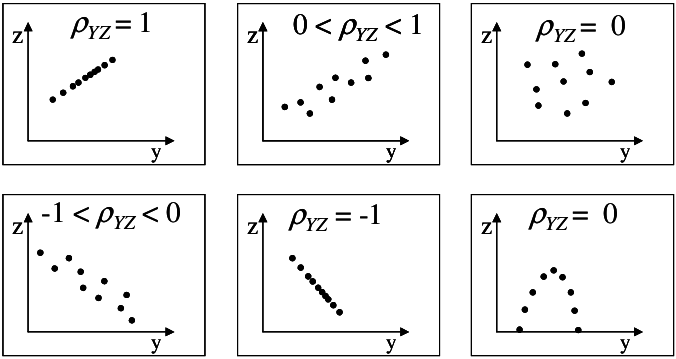
\includegraphics[width=0.95\textwidth]{fiBi213.png}
        \vspace{-0.1cm}
        \captionof{figure}{Scatter plots and $r_{X,Y}$ (taken from \cite{bierkens2007})}
\end{frame}




\begin{frame}[allowframebreaks]{References}
 \bibliographystyle{plainnat}
    \bibliography{references}
\end{frame}
\end{document}
